\section{Tools and Data}
Every year technology for generating and measuring particle collisions is improved. 
As a consequence, the amount of data increases drastically. The ATLAS experiment
is one of the largest particle detector experiments currently operating at the 
CERN laboratory near Geneva. ATLAS alone generates approximately 1 petabyte of raw
data every second from proton-proton collisions at the \ac{LHC}. 
With amounts of data this large, data handling and storing is a big challenge. 
Therefore, taking advantage of sophisticated numerical tools and data frameworks is
pivotal if scientific development is to keep up with technological development.
\\
In this section I will cover some tools and frameworks I have used to 
complete my analysis. Large amounts of details and explanations will not be covered. 
Instead, this section will highlight which tools were used and some motivation
for choosing them. Additionally, I will cover some details regarding the data
being used, both \ac{MC} and real.
\subsection{Monte Carlo Data}
\subsection{ROOT, RDataframe and Pandas}
ROOT \cite{ROOT} is at its core a large $C{++}$ library and data structure made specifically for big data
analysis and computing, as well as data visualization. Today, all ATLAS data is stored as a ROOT-file along
with more than 1 exabyte of data worldwide. ROOT has many \ac{HPC} qualities which makes it ideal for particle
physics analysis which demands heavy computations. Additionally, many particle physics-specific packages
have been developed to make it an even better tool. Any function not already in library,
can easily be added in a \ac{HPC}-effective manner through $C{++}$.
\\
All distribution plots made for this thesis were created using ROOT. ROOT has implemented a highly intuitive and
effective \ac{API} for data comparison and visualization. ROOT allows for quick and direct 
comparison between data through an advanced graphical user interface. Additionally, a lot of
functionality for creating complex stacked histogram are implemented in the ROOT \ac{API}, such
as uncertainty calculations and ordering of histograms. 
\\
As for the data structure, the raw data was loaded as a ROOT-file. To easier handle the data and add
new features, I used the RDataFrame structure \cite{RDataFrame}. RDataFrame allows for easy 
addition of new columns as well as filtering of events through native functionality. As a consequence
I used RDataFrame to calculate all higher-level features such as $M_{T2}$ and $M_{lll}$. An example is 
shown in the following section. 
\\
After all data handling was complete, I used ROOT's $AsNumpy$ function to translate the data frame as 
a numpy object, which then allowed me to transform it to a Pandas-data frame \cite{Pandas}. This is done
because Pandas, like most \ac{ML}-tools work in a strict Python environment. Pandas, similarly to RDataFrame
includes many deep computational libraries, and is optimal for analysis of big data. When all \ac{ML} is completed,
the data is transformed back to RDataFrame, to take advantage of plotting functionality in ROOT.

\subsection{Computing features in ROOT: Example}
In this section I will cover a simple example to highlight the steps taken in generating the dataset 
I used during analysis. As mentioned earlier, the two main frameworks used were RDataFrame and Pandas. 
In this example I will cover the case of a feature not already in the ROOT file, namely the trilepton
invariant mass. All loading of data is done using the ROOT framework and is quickly made into a 
RDataFrame. To effectively generate new features, we want to stay in ROOT and RDataFrame. Therefore,
we create our $C{++}$-file, \emph{helperfunction}. The helperfunction contains all additional 
ROOT function that are used in the analysis and is not already native to ROOT. In the case 
of computing the trilepton invariant mass, the $C{++}$-function is created like shown in 
\ref{lst:mlll}.
\\
In \ref{lst:mlll}, we see a couple of measures taken to uphold to the ROOT environment. The first is 
the typecasting to $VecF\_t$. $VecF\_t$ is created to wrap floats in the native ROOT vector object, $RVec$. 
The same is done in other cases such as float and integers, $VecI\_t$ and $VecB\_t$. The second measure
was using $TLorentzVector$ \cite{TLorentzVector} to calculate the invariant mass. $TLorentzVector$ is a class
native to ROOT with many built-in functions. In this case we use the class to create three vectors through the 
variables, $P_t$, $\eta$, $\phi$ and M. Then, through the $TLorentzVector$ class we can simply
add all three vector together, and extract the invariant mass. 
\lstset{style=Cpp}
\begin{lstlisting}[caption={$C{++}$-function for $M_{lll}$.},captionpos=b, label={lst:mlll}]
// Compute the trilepton invariant mass 
float ComputeInvariantMass(VecF_t& pt, VecF_t& eta, VecF_t& phi, VecF_t& m) {
  TLorentzVector p1;
  TLorentzVector p2;
  TLorentzVector p3;
  p1.SetPtEtaPhiM(pt[0], eta[0], phi[0], m[0]);
  p2.SetPtEtaPhiM(pt[1], eta[1], phi[1], m[1]);
  p3.SetPtEtaPhiM(pt[2], eta[2], phi[2], m[2]);
  return (p1 + p2 + p3).M();
}
\end{lstlisting}
With a helper function created in $C{++}$ we can move over to a Python and RDataFrame environment
for calculation and plotting. In the code written in \ref{lst:df_mlll}, I have shown a simple example 
of loading new $C{++}$-functions, filtering out bad events, calculating new features and adding said 
features to a histogram. The first three lines of code both process and include the helperfunction 
functions into the ROOT framework. Then I loop over all keys in the data frame, which in my case
are the different channels (i.e Diboson, $t\bar{t}$ etc.). For each channel I filter out 'good' events,
based on the criteria from section \ref{subsec:Cuts}. Then, I use RDataFrame's $Define$ function to calculate
and add a new feature using our $ComputeInvariantMass$-function. Finally, I save the feature as 
an $Histo1D$ object, which I plot later using ROOT plotting \ac{API}'s.
\lstset{style=Python}
\begin{lstlisting}[caption={Python-file for calling dataframe and calculating $M_{lll}$.},captionpos=b, label={lst:df_mlll}]
R.gROOT.ProcessLine(".L helperFunctions.cxx+");
R.gInterpreter.Declare('#include "helperFunctions.h"') 
R.gSystem.Load("helperFunctions_cxx.so")

for k in df.keys():
    # Define good leptons
    isGoodLepton = "feature1 < cut1 && feature2 >= cut2"

    # Define good leptons in dataframe
    df[k] = df[k].Define("isGoodLepton",isGoodLepton)

    # Define number of good leptons
    df[k] = df[k].Define("nGoodLeptons","ROOT::VecOps::Sum(isGoodLepton)")

    # Demand 3 good leptons 
    df[k] = df[k].Filter("nGoodLeptons == 3")

    # Define Invariant Mass (lll)
    df[k] = df[k].Define("mlll","ComputeInvariantMass(lepPt[isGoodLepton], 
                                                      lepEta[isGoodLepton], 
                                                      lepPhi[isGoodLepton], 
                                                      lepM[isGoodLepton])")
    # Add to histogram
    histo["mlll_%s"%k] = df[k].Histo1D(("mlll_%s"%k,
                                        "mlll_%s"%k,40,50,500),
                                        "mlll",
                                        "wgt_SG")     
\end{lstlisting}
In this example I chose the trilepton invariant mass, but in the analysis all high-level features were
calculated using a similar method. The workflow of the method is visualized in figure \ref{fig:WF}. We
load data in ROOT format, data handling and plot feature distrobution  in RDataFrame, perform \ac{ML}-
analysis in Pandas and plot results in RDataFrame.
\begin{figure}
    \centering
    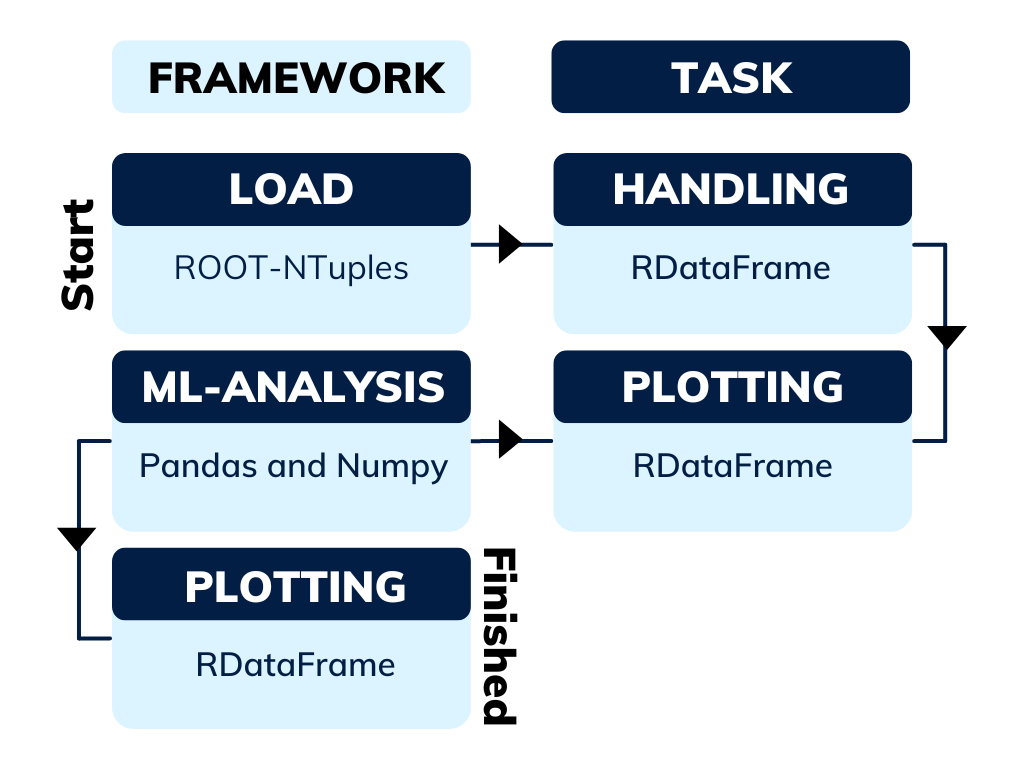
\includegraphics[width=0.7\textwidth]{Figures/Illustrations/TaskFlow.png}
    \caption{A visual summary of the workflow and framework use for the 
    computational analysis. }
    \label{fig:WF}
\end{figure}

